\documentclass{article}
\usepackage[dvipsnames]{xcolor}
\usepackage{amsmath}
\usepackage{graphicx}
\usepackage{enumitem}
\usepackage{centernot}
\usepackage{setspace}
\usepackage[margin=0.95in]{geometry}
\usepackage{titling}

\setlength{\droptitle}{-7em}   % This is your set screw

\begin{document}

\title{Philosophy of Physics\\ Midterm}
\author{Ozaner Hansha}
\date{March 10, 2020}
\maketitle

\subsection*{Question 1}
\noindent\textbf{Prompt:}  Compare and contrast the standard conception of time reversal invariance with Albert’s conception. Why does Albert reject the standard view? Why does he nonetheless agree with the standard view that Newtonian mechanics is time reversal invariant.
\bigskip

\noindent\textbf{Response:} For a theory to be time-reversal invariant (TRI) under Albert's conception, we must have that for any valid set of consecutive states of a system:

$$\underbrace{S_1,S_2,\cdots S_n}_{\text{is valid}}\implies \underbrace{S_n',\cdots,S_2',S_1'}_{\text{is valid}}$$

Where the $'$ operator is defined as:

$$S_i'\equiv S_i\text{ with all particle velocities reversed.}$$

Note that reversing all velocities also correspondingly affects other time based quantities. For example, momentum will also be reversed as it is the product of mass and (a reversed) velocity.
\smallskip

In contrast, the standard view of TRI is similar:

$$\underbrace{S_1,S_2,\cdots S_n}_{\text{is valid}}\implies \underbrace{S_n^*,\cdots,S_2^*,S_1^*}_{\text{is valid}}$$

But this time the $^*$ operator changes more than just velocity. It can also reverse other quantities such that the sequence follows the theory's dynamics. Albert portrays it as an unprincipled approach.

As it turns out though, both conceptions are equivalent when it comes to Newtonian mechanics as the only quantity the standard view needs to reverse (and the only quantity available to reverse really) is velocity:

$$\underbrace{S_i'=S_i^*}_{\text{Newtonian Mechanics}}$$

Moreover, both operators do indeed satisfy their respective definitions of TRI:

$$\underbrace{S_1,S_2,\cdots S_n}_{\text{is valid}}\implies\underbrace{S_n',\cdots,S_2',S_1'}_{\text{is valid}}=\underbrace{S_n^*,\cdots,S_2^*,S_1^*}_{\text{is valid}}$$
\smallskip

This isn't the case with other theories though. For example, in classical electrodynamics the $^*$ operator reverses not just the velocities of the particles but also the direction of magnetic fields. In contrast the $'$ operator still only reverses velocities and since the strength of a magnetic field is not dependent on any velocity, we have that:
$$\underbrace{S_i'\not=S_i^*}_{\text{Classical Electrodynamics}}$$
\smallskip

And moreover that classical EM only satisfies TRI under the standard conception due to the affect of magnetic fields:
\begin{align*}
  \underbrace{S_1,S_2,\cdots S_n}_{\text{is valid}}&\centernot\implies\underbrace{S_n',\cdots,S_2',S_1'}_{\text{is valid}}\tag{Albert's TRI}\\
  \underbrace{S_1,S_2,\cdots S_n}_{\text{is valid}}&\implies\underbrace{S_n^*,\cdots,S_2^*,S_1^*}_{\text{is valid}}\tag{Standard TRI}
\end{align*}
\newpage

\setstretch{1.4}


\subsection*{Question 2}
\noindent\textbf{Prompt:} Explain why Arntzenius calls the calculus-based conception of instantaneous velocity a ``neighborhood quantity." Then explain the ``impetus view" of velocity that he discusses. Finally, raise an objection to one of these views of velocity (either one).
\bigskip

\noindent\textbf{Response:} Arntzenius calls the calculus-based conception of instantaneous velocity a ``neighborhood quantity" because in this view, velocity is not a fundamental property of particles, only position is. And since velocity is commonly formulated as simply the time derivative of position, we can recover the instantaneous velocity of a particle at any time $t^*$ given $x(t)$ on a finite (or infinitesimal) neighborhood around $t^*$. By `neighborhood', we of course mean some interval of time $[t^*-\epsilon,t^*+\epsilon]$ where $\epsilon$ may be finite or infinitesimal (but not 0). Using the values of $x(t)$ over such a neighborhood we are able to calculate the derivative of the particle's position, i.e. instantaneous velocity $v(t^*)$,  for any such $t^*$.

The impetus view holds that all matter has an additional kinematic property that informs its future motion at every instant: impetus. Under this view, the state of a particle consists of not just its position, but an `intrinsic velocity'. This intrinsic velocity is simply the aforementioned impetus divided by the mass of the particle, which is a static rather than kinematic property.

It is important to note that, unlike the `at-at' view of velocity which makes use of the aforementioned notion of a neighborhood based instantaneous velocity, the intrinsic velocity of a particle in the impetus view is not a derived quantity. As such, we must include another law-like statement (what Arntzenius calls an ``additional ontology") that states that the intrinsic velocities always happen to be equal to the derivatives of the position of the object. Without this law, we could not rule out situations where the velocities \textit{don't} coorespond to the derivative of the position over time.
\bigskip

In light of this, we can now identify a key objection to the at-at view: that it lacks the sort of casual explanatory power that other theories of motion possess. This is because, in an at-at world, position is the only real kinematic quantity. While we can calculate the velocity of a particle given a neighborhood and then use that velocity to predict its future behavior, that neighborhood certainly cannot be the \textit{cause} of its motion. The neighborhood of $x(t)$ around some time $t^*$ includes, even if just infinitesimally, the particle's future position. And certainly the future position of the particle cannot depend, even if just partially, on itself.

Contrast this with the impetus view that holds that the impetus (essentially momentum) of an object at an instant, along with its position, is what determines its future behavior. That said, there are ways to avoid this problem in the at-at view but only by abandoning our normal conceptions of determinism as based on instants of time among other things.
\newpage

% \subsection*{Question 4}
% \noindent\textbf{Prompt:} Explain Hutchison’s argument that Newtonian mechanics is not time reversal invariant. Then raise an objection to Hutchison’s argument.
% \bigskip

% \noindent\textbf{Response:} 

\subsection*{Question 5}
\noindent\textbf{Prompt:}  Explain why the example of either the space invaders or Norton’s dome seems to show that Newtonian mechanics is an indeterministic theory. Then raise an objection to the argument based on that example.
\bigskip

\noindent\textbf{Response:} Consider a Newtonian particle accelerating in such a way as to have its velocity asymptote at some time $t^*$, in effect blowing up to infinity in finite time. Such a scenario has been shown to be possible by Xia \cite{infiniteaccel} with just 5 innocuously positioned particles that act on each other via gravity.

\begin{center}
  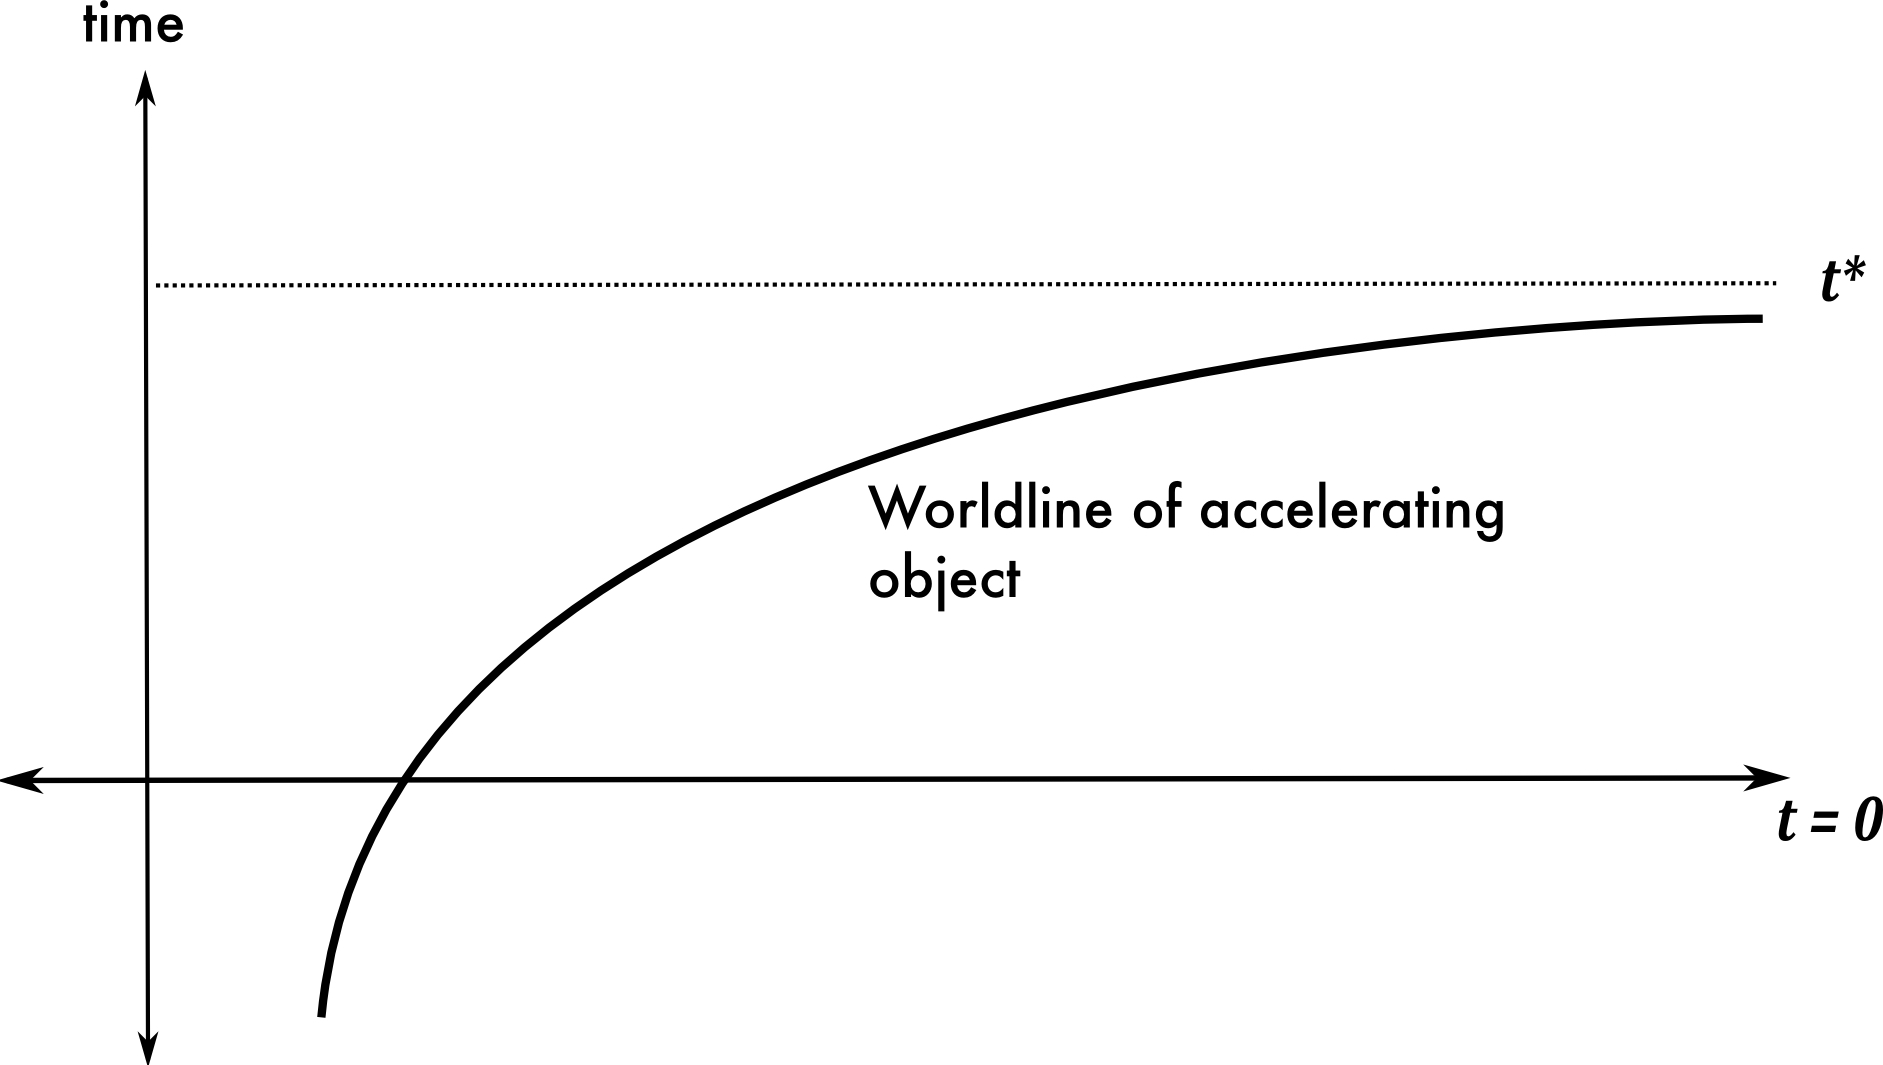
\includegraphics[scale=0.2]{disappearer.jpg}  
\end{center}

As we can see in the above space vs time graph \cite{spacegraph}, the particle's position grows unbounded as $t\to t^*$ and once $t=t^*$ we find that the particle has `escaped the universe.' After this point the particle no longer exists in the universe. While this is certainly unsetteling, it is not obvious that determinism has been violated yet as the universe seems to evolve in the same way as before (sans one particle).

However recalling that Newtonian mechanics (NM) is time-reversable, the time reverse scenario should also be equally valid under NM. The time reverse being a particle simply appearing in our universe after some time $t^*$ from `spacial infinity':

\begin{center}
  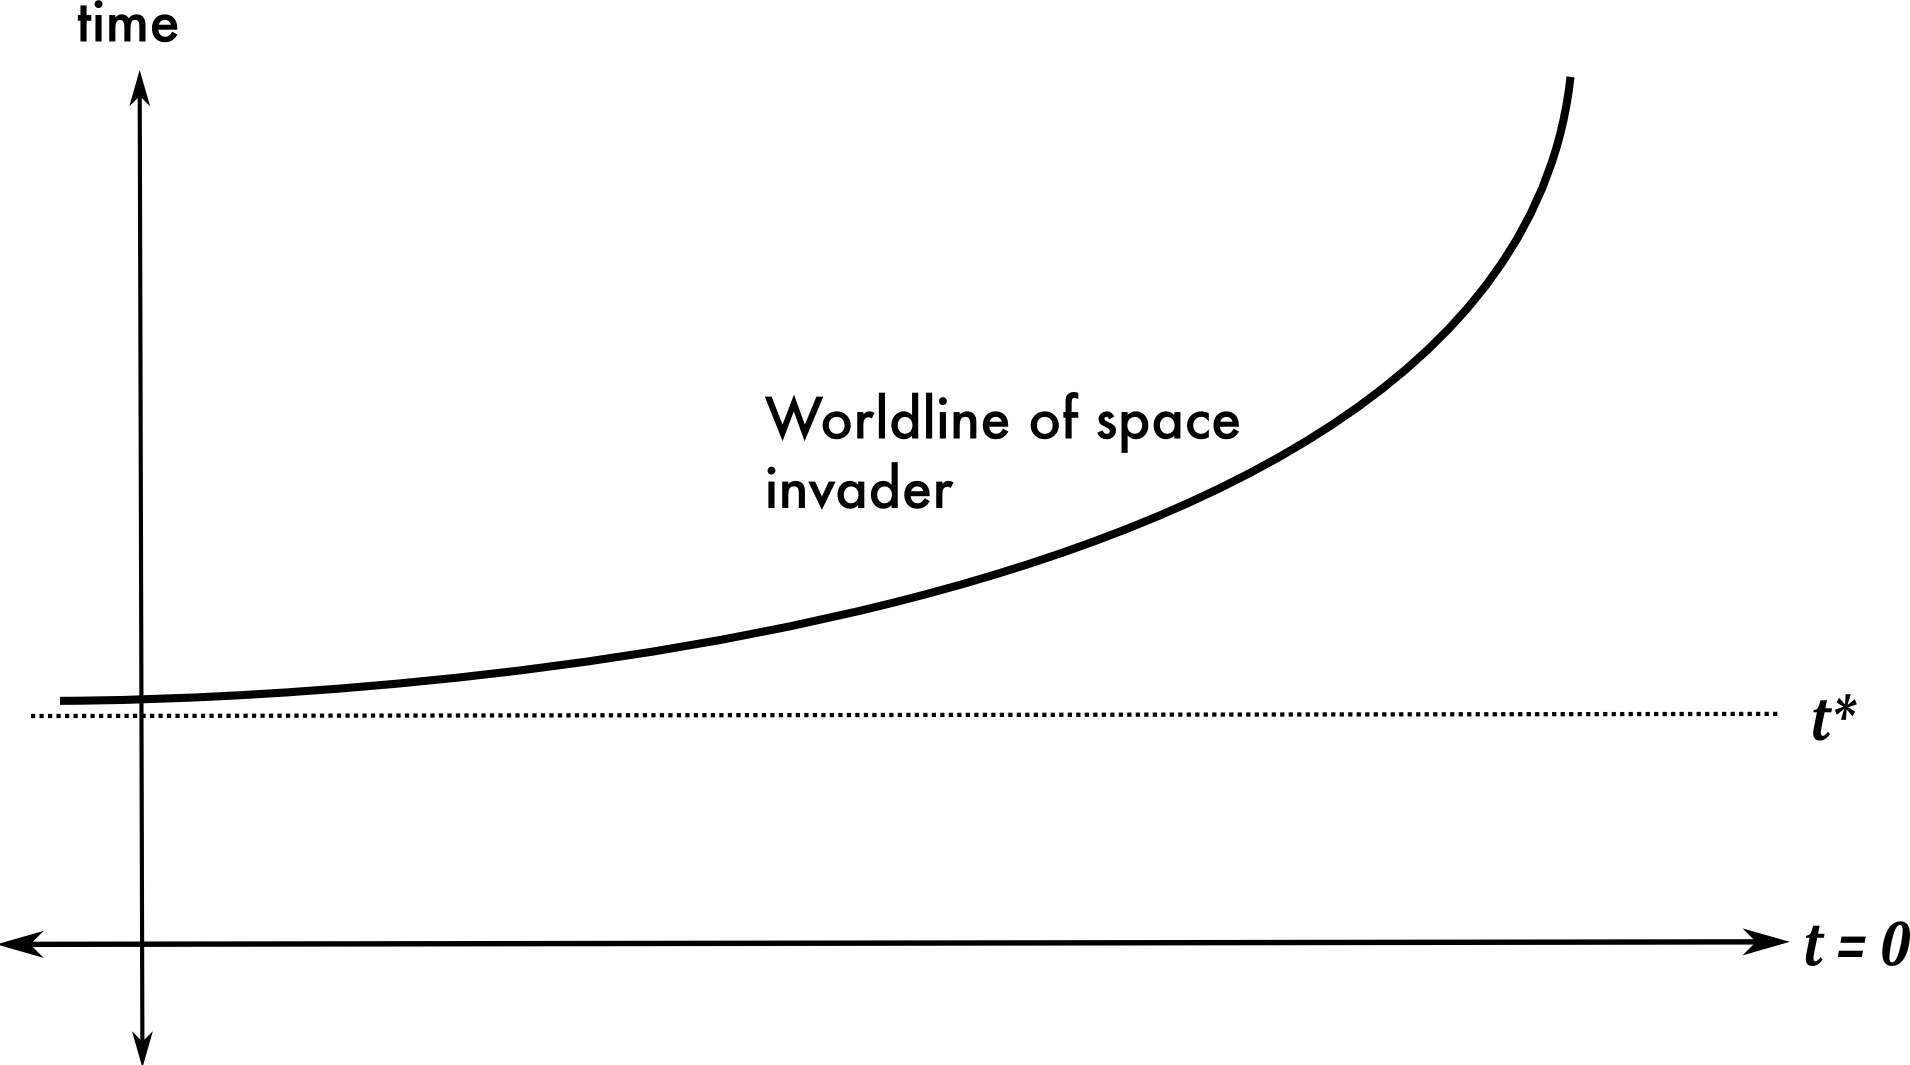
\includegraphics[scale=0.18]{space-invader.jpg}  
\end{center}

And since NM is invariant to relative time changes, i.e. it is not dependent on absolute time, a particle could swoop down from infinity not just at time $t^*$ but at any time before or after. We dub such particles ``space-invaders".

And so by the existence of space-invaders, we have shown that it is perfectly consistent with NM, and its time-reversibility, that a particle can simply appear in space. This violates determinism in that the current state of the universe at, say, time $t^*$ does not tell us, under $F=ma$, what the state of the universe will be like after this time. Specifically because it will miss the appearance of the space-invader.

While this scenario is a good counterpoint regarding the commonly held belief that NM is deterministic, note it crucially depends on the assertion that NM is time-reversable. Without this property the existence of space-invaders cannot be shown. We still can have particles that disappear from the universe, but such particles do not violate determinism as the entire state of the universe can still be predicted without them (since they left the universe and are never coming back).

And so it would seem that we can save our belief that NM is deterministic, at least from this argument, if we give up its time-reversability.
\newpage

\subsection*{Question 6}
\noindent\textbf{Prompt:} Describe the thought experiment of Maxwell’s demon. What does this thought experiment seem to show about thermodynamics (the second law in particular)? Explain.
\bigskip

\noindent\textbf{Response:} Consider a gas filled box with two chambers $A$ and $B$, with one being hotter than the other, and both being seperated by a small slit \cite{demon pic}:

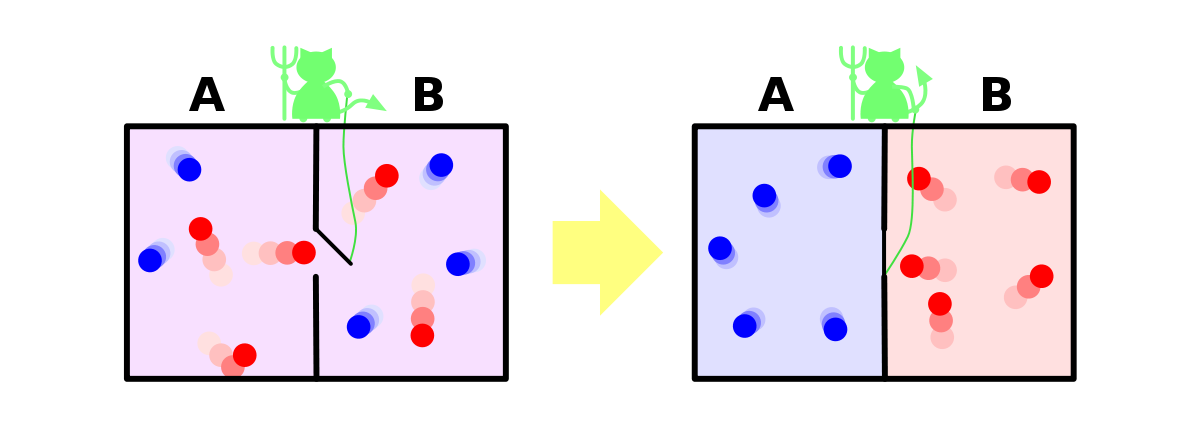
\includegraphics[width=\linewidth]{mdemon.png}

The second law of thermodynamics tells us that the temperature gradient of the box should diffuse over time, as opposed to maintaining its sharp temperature difference or even having the temperature difference grow further.

Now imagine that we add a controllable shutter in place of the slit and have an entity, the so called demon, that can observe the velocities of particles that are nearing the slit and decide to let them through or not by controlling the shutter.

If the demon so desired, it could only allow particles from $A$ to travel to $B$ if they had a higher than average velocity and vice versa for particles from $B$ to $A$. Such a scenario would have, counter to the second law, the boxes not just maintaining their temperature difference but infact increasing it.

This thought experiment raises the concern that the so called second \textit{law} of thermodynamics may not hold in certain cases, like the one mentioned above. Clearly entropy is \textit{not} increasing over time in this scenario.

That said, there are obvious objections to the legitmacy of the above though experiment, especially equipped with a modern understanding of entropy and statistical mechanics. Even putting aside the question of acquiring such a `demon' that could somehow measure the velocities of incoming particles and operate a particle sized shutter, it has been argued that such a demon would itself increase the entropy of the system, by way of operating the shutter and computing when to switch said shutter.

While this is certainly problamatic, that same modern physics allows us to entirely bypass the invocation of the demon in the first place. Indeed we know, absent any information of the particular velocities or positions of the particles in either chamber, that a variety of microstates are compatible with the macrostate of each chamber having some measured temperature. We also know that while most, for some reasonable formalism of `most', of these microstates eventually evolve into microstates compatible with a macrostate with higher entropy, there are still some microstates that just so happen to evolve to be compatible with lower entropy macrostates.

Put another way, given a box with particles of random position and velocities, it is entirely possible, however unlikely, that these particles are set up in such a way as to evolve over time to a configuration where most of the high velocity particles are in one chamber (making it hotter) and the low velocity ones in another (making it cooler).

Indeed this reasoning allows us to arrive at a more refined version of our above conclusion. Namely that the second law is not just fallable, but more specifically that it is only highly probable. That, given some scenario, there is a very small chance that it may not hold. Making it seem like less of a \textit{law} and more of a statistical statement.
\newpage

\subsection*{Question 8}
\noindent\textbf{Prompt:} You enter a room that no one else has been in for a while. You find a small ice cube floating in a cup of water. You expect that in 30 minutes (if no one interferes), the ice will have melted to an even smaller cube. You think that 30 minutes ago, there had been a larger ice cube. How does Albert account for this asymmetric inference?
\bigskip

\noindent\textbf{Response:} Let us first examine the forward direction. Given a macrostate of the ice-glass-environment system, i.e. average temperature of the components, pressure, etc., there are a variety of particular configurations, or microstates, compatible with it. It can be shown that most, in a somewhat reasonable measure-theoretic sense, of these microstates tend towards a higher overall entropy. Equipped with the statistical postulate, which states that our particular system is uniformly likely to be any one of the compatible microstates, this implies that our particular system is highly likely to increase in entropy. This in turns cooresponds to the temperature of the system becoming more diffuse and the ice melting, netting us our prediction.

While this does accurately describe our experience and observation of systems and their entropy over time, it leads us to a problem. The above reasoning is time reversable, which is to say systems in the past are predicted to be just as high entropy as those in the future. This is clearly counter to our observation which shows that entropy was lower in the past and has increases over time, hence our prediction that the ice cube used to be larger (i.e. the system had less entropy).

Albert accounts for this asymmetry via the past hypothesis. Essentially, we posit that the initial state of the universe (or at least a state far enough before our observational capacity) was in a state of low entropy. This allows us to rid ourselves of the, all things being equal, much more likely possibility that the past had a higher entropy that the statistical postulate implies. Indeed if the universe was originally in such a state, the increase of entropy over time (and thus decrease backwards in time) is the most probable outcome and indeed the one we observe.

\vspace{10em}

\begin{thebibliography}{999}
    \bibitem{demon pic}
      Maxwell's demon diagram.\\
      https://commons.wikimedia.org/wiki/File:Maxwell\%27s\_demon.svg
    \bibitem{infiniteaccel}
      Off to Infinity in Finite Time.\\
      \emph{Notices of the AMS}, Xia 1993.
    \bibitem{spacegraph}
      Space-Invader graphs\\
      https://plato.stanford.edu/entries/determinism-causal/
\end{thebibliography}
\end{document}